\section[Migrations of $\xi$]{Migrations in $\mathbf{\xi}$}\label{section:star_xi}
The analysis was performed in three ranges of $\xi$. Thus, there are
migrations into and out of these $\xi$ regions. They mainly originate from the resolution of $\xi$ reconstructed from RP tracks. Figure~\ref{fig:xi_correction_resolution} shows the resolution of $\xi$ as a function of the true-level $\xi$ (denoted as $\xi_\textrm{true}$) with fitted zeroth order polynomial. The resolution of $\xi$ is fairly constant and equals to about $0.3\%$.

The corrections due to migrations into and out of  $\xi$ regions was defined as:
 \begin{equation}
 f_{\xi} = \frac{1-f_{\xi}^-}{1-f_{\xi}^+}
 \end{equation}
 where:
 \begin{description}
 	\item $f_{\xi}^-$ is the fraction of events for which the corresponding true-level $\xi_\textrm{true}$, is outside of the~$\xi$ region,
 	\item $f_{\xi}^+$  is the fraction of events for which the corresponding reconstructed $\xi_\textrm{reco}$ is outside of the $\xi$ region.
 \end{description}
 \begin{figure}[h!]
 	\centering
 	\begin{subfigure}{.49\textwidth}
 		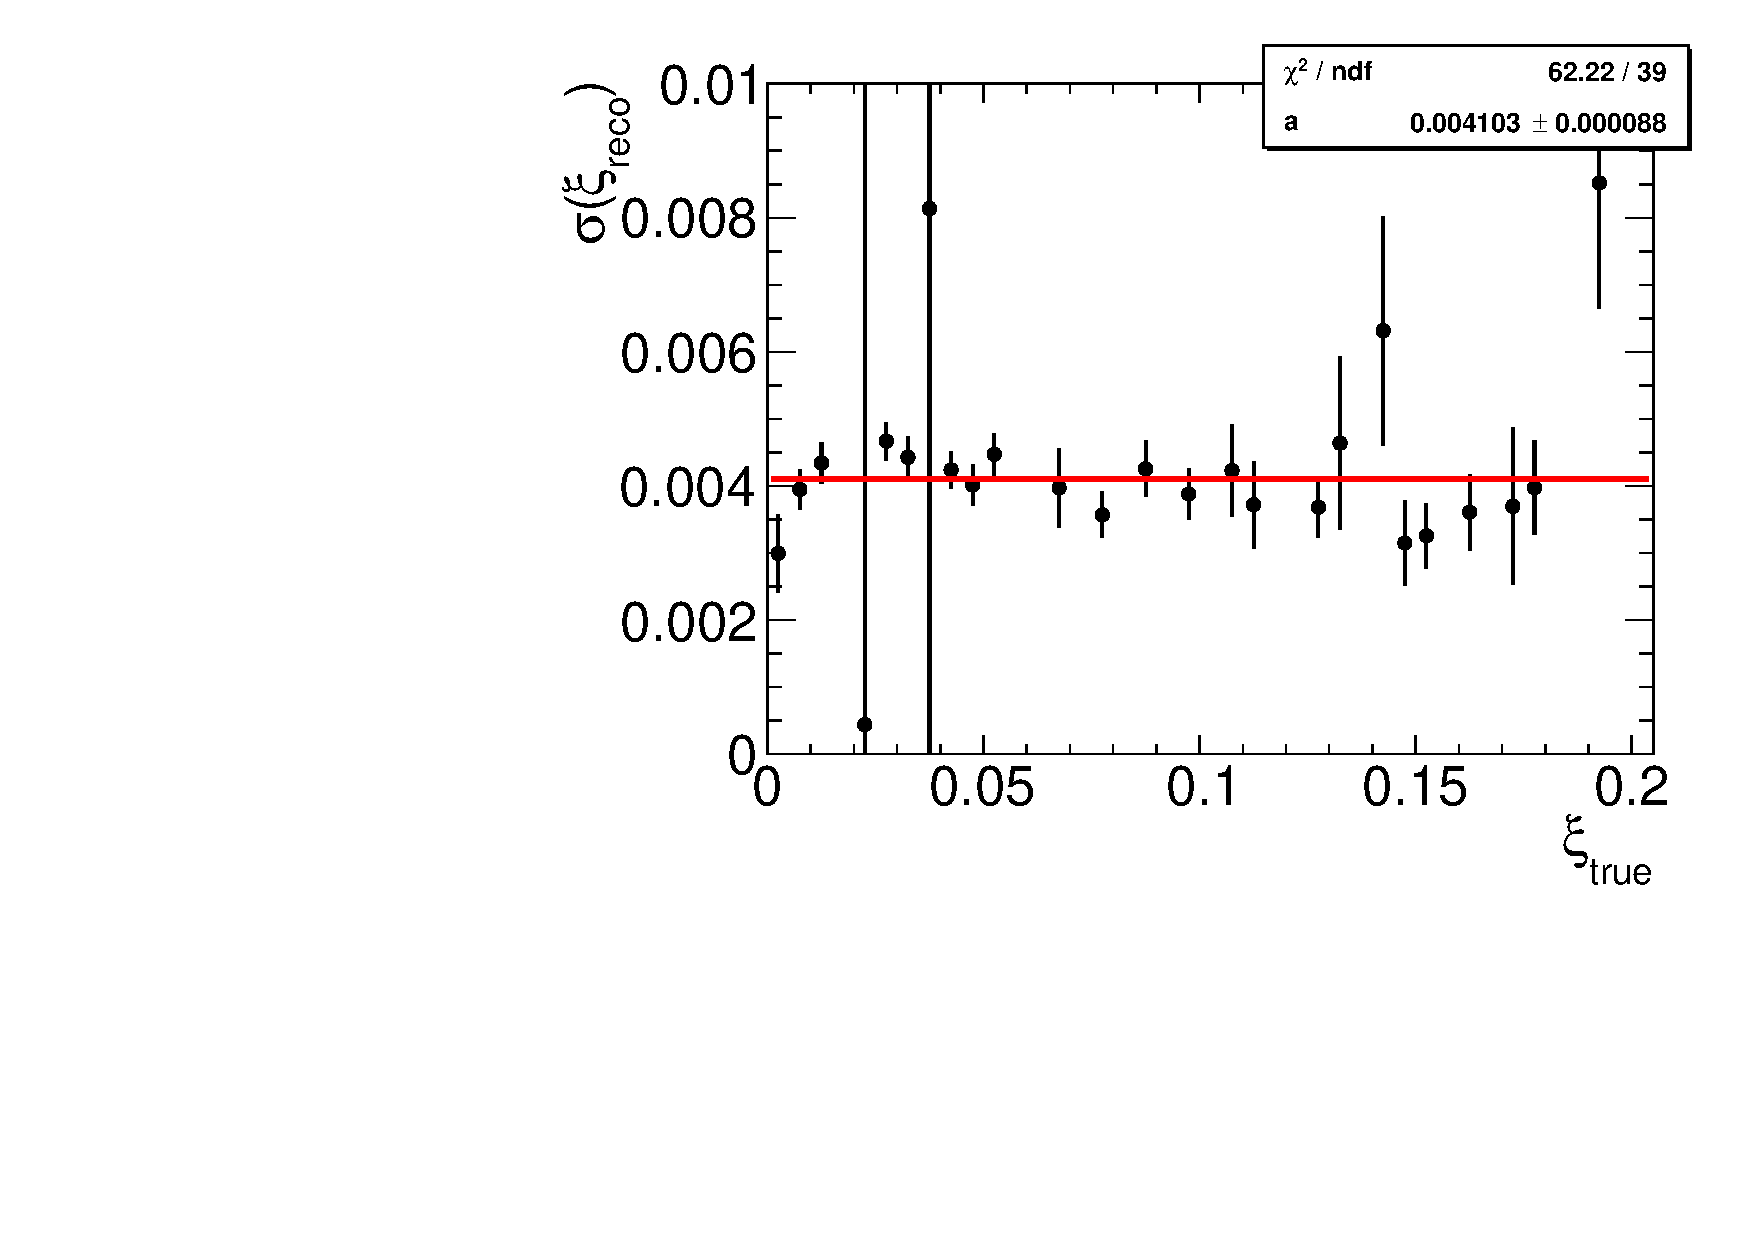
\includegraphics[width=\textwidth,page=1]{chapters/chrgSTAR/img/xiMigration/RPresolution.pdf}
 	\end{subfigure}
 	\begin{minipage}{.49\textwidth}
 		\caption{The resolution of $\xi$ as a function of $\xi_\textrm{true}$. The zeroth order polynomial, shown as red line, was fitted.}
 		\label{fig:xi_correction_resolution}
 	\end{minipage}
 \end{figure}
 \begin{figure}[h!]
 	\centering
 	\begin{subfigure}{.49\textwidth}
 		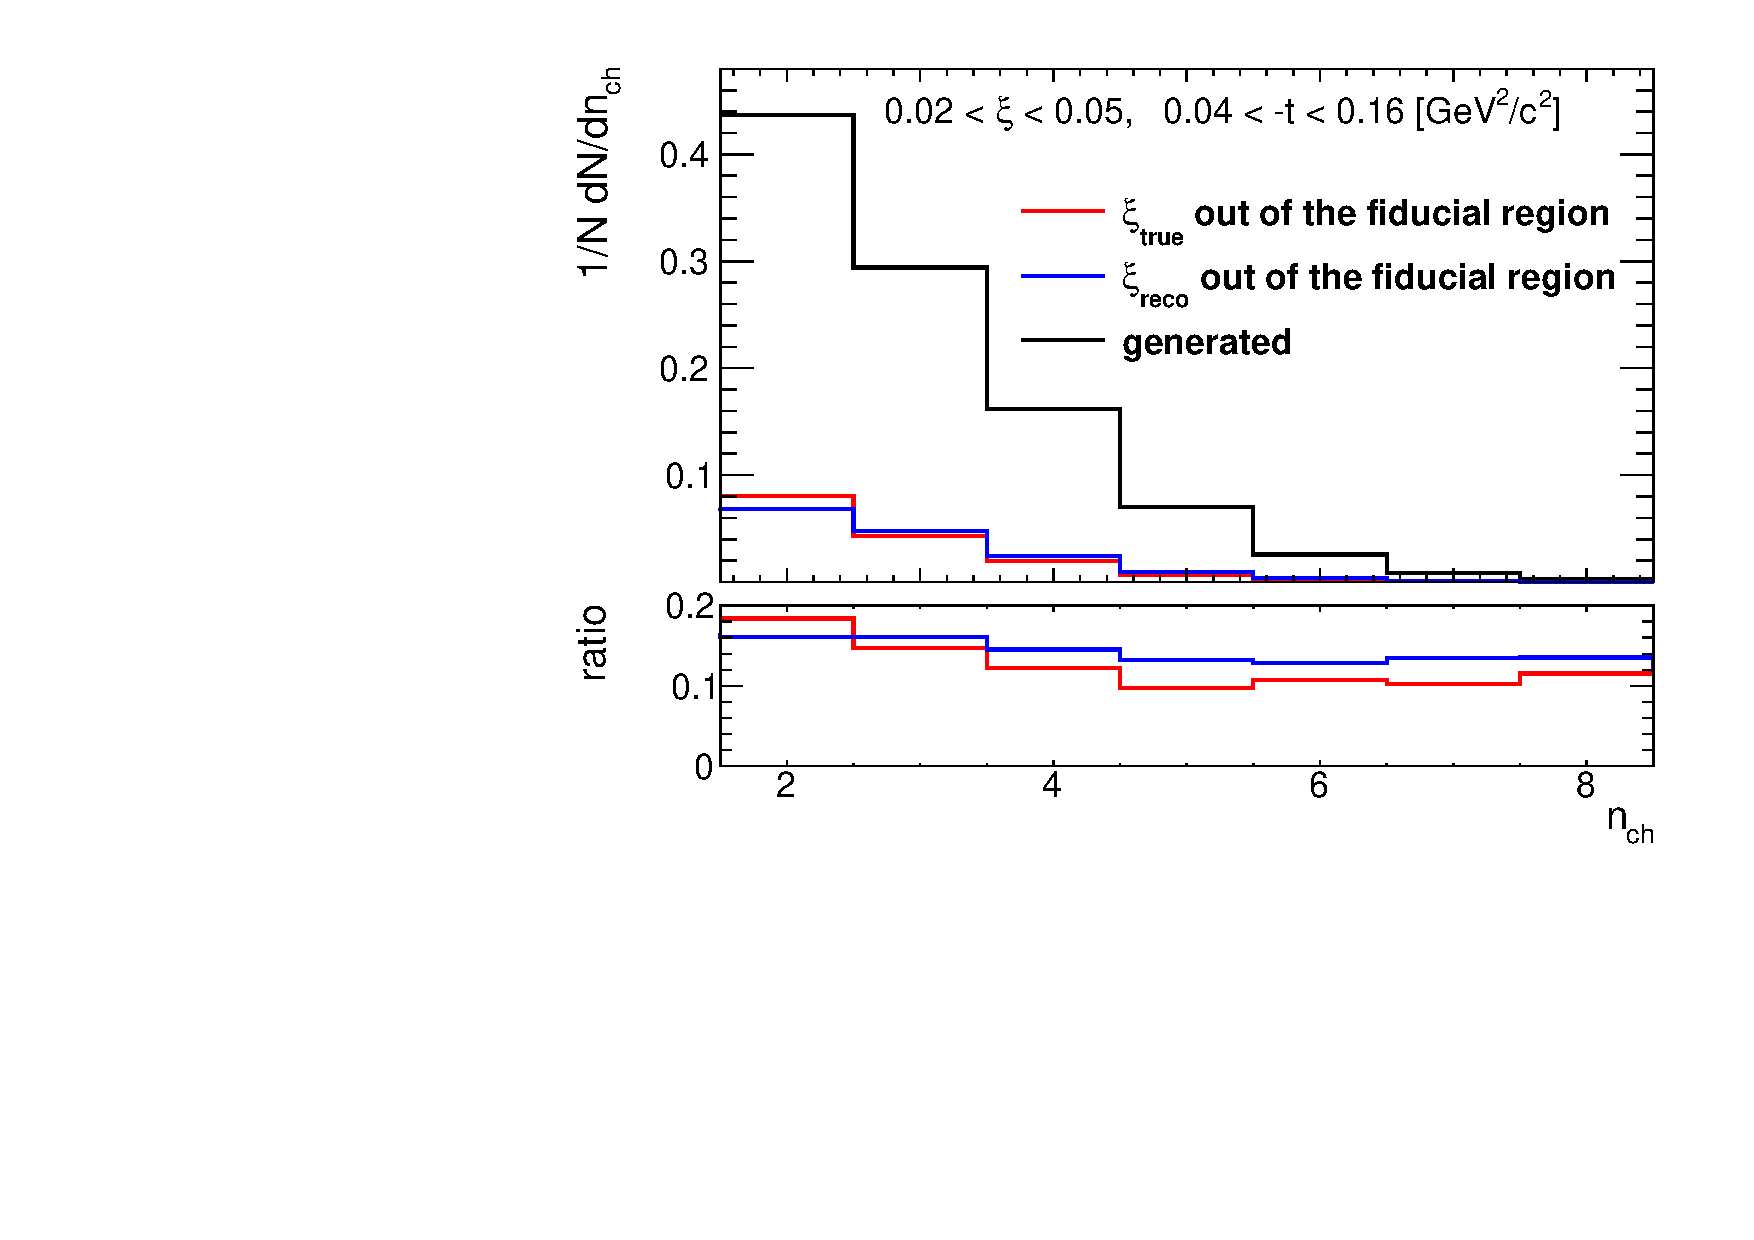
\includegraphics[width=\textwidth,page=1]{chapters/chrgSTAR/img/xiMigration/xi.pdf}
 	\end{subfigure}
 	\begin{subfigure}{.49\textwidth}
 		\includegraphics[width=\textwidth,page=2]{chapters/chrgSTAR/img/xiMigration/xi.pdf}
 	\end{subfigure}
 	\begin{subfigure}{.49\textwidth}
 		\includegraphics[width=\textwidth,page=3]{chapters/chrgSTAR/img/xiMigration/xi.pdf}
 	\end{subfigure}
 	\begin{minipage}{.49\textwidth}
 		\caption{Fraction of events (red) $f_{\xi}^-$ and (blue)  $f_{\xi}^+$ as a function of $n_\textrm{ch}$ in three ranges of $\xi$.}
 		\label{fig:xi_correction_nch}
 	\end{minipage}
 	
 \end{figure}
 
 The $f_{\xi}$ was calculated for each measured variable separately. \Cref{fig:xi_correction_nch,fig:xi_correction_pt,fig:xi_correction_eta} show the fraction of events $f_{\xi}^-$ and $f_{\xi}^+$ as a function of $n_\textrm{ch}$, $p_\textrm{T}$ and $\bar{\eta}$. The lower panel in each figure shows the~corresponding correction factor $f_\xi$. The largest differences between migrations into and out of the $\xi$ regions were observed at $0.02<\xi<0.05$, where they are of the order of $2-4\%$. In the other $\xi$ regions, the difference between $f_{\xi}^-$ and $f_{\xi}^+$  is smaller than $1\%$.
\begin{figure}[h!]
	%\vspace{-0.7cm}
	\thisfloatpagestyle{empty}
	%\vspace{-2.5cm}
	\centering
	\begin{subfigure}{.49\textwidth}
		\includegraphics[width=\textwidth,page=4]{chapters/chrgSTAR/img/xiMigration/xi.pdf}
	\end{subfigure}
	\begin{subfigure}{.49\textwidth}
		\includegraphics[width=\textwidth,page=5]{chapters/chrgSTAR/img/xiMigration/xi.pdf}
	\end{subfigure}
	\begin{subfigure}{.49\textwidth}
		\includegraphics[width=\textwidth,page=6]{chapters/chrgSTAR/img/xiMigration/xi.pdf}
	\end{subfigure}
	\begin{minipage}{.49\textwidth}
		\caption{(red) Fraction of events $f_{\xi}^-$ and (blue) $f_{\xi}^+$  as a function of $p_\textrm{T}$ in three ranges of $\xi$.}
		\label{fig:xi_correction_pt}
	\end{minipage}
	%\vspace{-0.5cm}
\end{figure}

\begin{figure}[h!]
	%\vspace{-0.5cm}
	\centering
	\begin{subfigure}{.49\textwidth}
		\includegraphics[width=\textwidth,page=7]{chapters/chrgSTAR/img/xiMigration/xi.pdf}
	\end{subfigure}
	\begin{subfigure}{.49\textwidth}
		\includegraphics[width=\textwidth,page=8]{chapters/chrgSTAR/img/xiMigration/xi.pdf}
	\end{subfigure}
	\begin{subfigure}{.49\textwidth}
		\includegraphics[width=\textwidth,page=9]{chapters/chrgSTAR/img/xiMigration/xi.pdf}
	\end{subfigure}
	\begin{minipage}{.49\textwidth}
		\caption{(red) Fraction of events $f_{\xi}^-$ and (blue) $f_{\xi}^+$  as a function of $\bar{\eta}$ in three ranges of $\xi$.}
		\label{fig:xi_correction_eta}
	\end{minipage}
	\vspace{-2.5cm}
	
\end{figure}